
\clearpage

% ===========================================================================
% 5. ARCHITECTURE
% ===========================================================================
\section{Architecture g\'en\'erale}

\subsection{Vue d'ensemble}

La plateforme fonctionne comme un ensemble de services Docker
interconnect\'es : un pipeline Celery (coupl\'e \`a RabbitMQ et Redis) scanne
le r\'eseau, enrichit et note les vuln\'erabilit\'es ; les r\'esultats sont
index\'es dans la stack ELK et les tickets sont ouverts dans GLPI. La gestion
des agents est assur\'ee par un serveur Fleet. Le sch\'ema suivant r\'esume
les composants et leurs relations :

\begin{figure}[htbp]
\centering
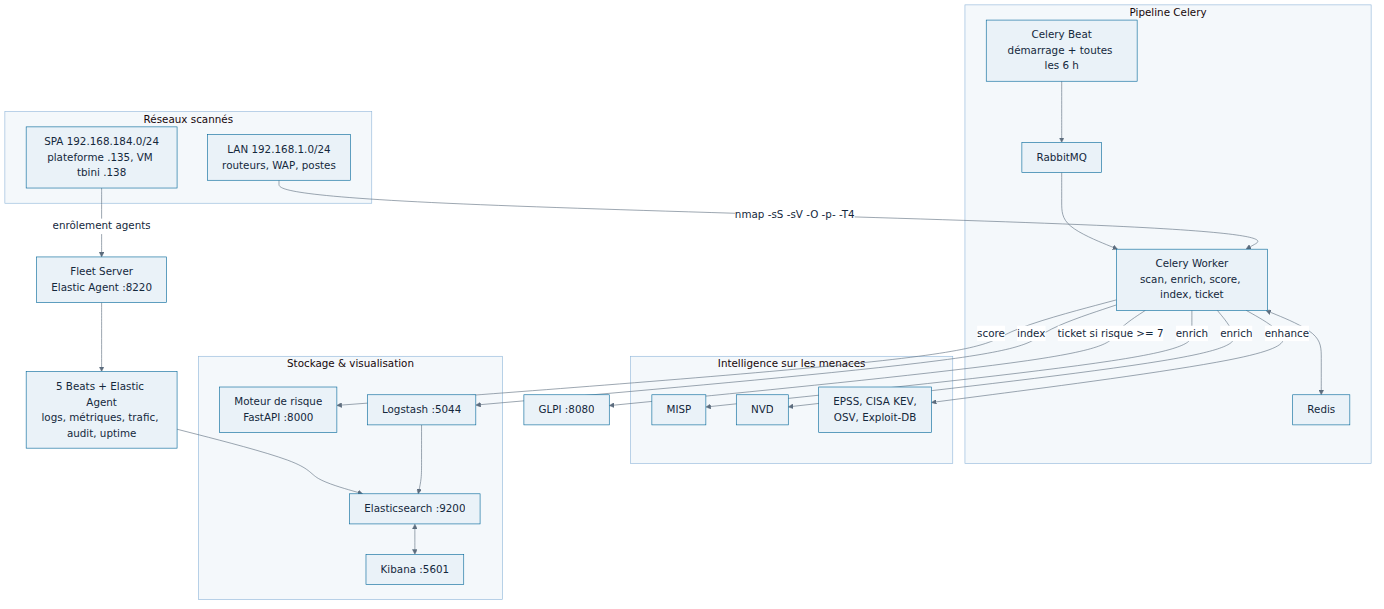
\includegraphics[width=0.72\linewidth,keepaspectratio]{diagrams/architecture.png}
\caption{Architecture g\'en\'erale de la plateforme VOC}
\end{figure}

\subsection{Gestion centralis\'ee des agents (Fleet)}

Une des \'evolutions majeures du projet a \'et\'e l'ajout du serveur
\textbf{Fleet Server} (Elastic Agent d\'edi\'e, port \texttt{:8220}). Il
permet :

\begin{itemize}[leftmargin=1.6em]
  \item d'enr\^oler des \textbf{agents externes} (h\^otes Linux/Windows hors
        Docker) avec des politiques d\'edi\'ees (\texttt{linux\_hosts},
        \texttt{windows\_hosts}) ;
  \item de centraliser la configuration des collecteurs (int\'egrations
        syst\`eme, logs, m\'etriques) ;
  \item de superviser l'\'etat de chaque agent depuis Kibana.
\end{itemize}

L'image Kibana a \'et\'e personnalis\'ee pour injecter les cl\'es de
chiffrement n\'ecessaires (\texttt{encryptedSavedObjects},
\texttt{security} et \texttt{reporting}), ce qui a \'elimin\'e les erreurs de
d\'emarrage et les \'ecrans de connexion fonctionnellement bloqu\'es.

\subsection{Services et ports}

\begin{center}
\small
\begin{longtable}{@{}l l l c@{}}
\toprule
\textbf{Service} & \textbf{Conteneur} & \textbf{Image} & \textbf{Port} \\
\midrule
\endhead
\bottomrule
\endlastfoot
RabbitMQ & \texttt{voc-rabbitmq} & \texttt{rabbitmq:3.12-management-alpine} & 5672, 15672 \\
Redis & \texttt{voc-redis} & \texttt{redis:7-alpine} & 6379 \\
Elasticsearch & \texttt{voc-elasticsearch} & \texttt{elasticsearch:8.11.0} & 9200 \\
Logstash & \texttt{voc-logstash} & \texttt{logstash:8.11.0} & 5044, 9600 \\
Kibana & \texttt{voc-kibana} & \texttt{kibana:8.11.0} (custom) & 5601 \\
Fleet Server & \texttt{voc-fleet-server} & \texttt{elastic-agent:8.11.0} & 8220 \\
MariaDB (GLPI) & \texttt{voc-mariadb} & \texttt{mariadb:10.6} & 3306 \\
MariaDB (MISP) & \texttt{voc-misp-db} & \texttt{mariadb:10.6} & -- \\
Moteur de risque & \texttt{voc-risk-engine} & custom (FastAPI) & 8000 \\
GLPI & \texttt{voc-glpi} & \texttt{diouxx/glpi:latest} & 8080 \\
MISP & \texttt{voc-misp} & \texttt{ghcr.io/misp/misp-docker/misp-core} & 8443 \\
Worker Celery & \texttt{voc-celery-worker} & custom (Python + nmap, root) & -- \\
Beat Celery & \texttt{voc-celery-beat} & custom (Python + nmap) & -- \\
Filebeat & \texttt{voc-elastic-agent} & \texttt{filebeat:8.11.0} & -- \\
Packetbeat & \texttt{voc-packetbeat} & \texttt{packetbeat:8.11.0} & -- (h\^ote) \\
Auditbeat & \texttt{voc-auditbeat} & \texttt{auditbeat:8.11.0} & -- \\
Metricbeat & \texttt{voc-metricbeat} & \texttt{metricbeat:8.11.0} & -- \\
Heartbeat & \texttt{voc-heartbeat} & \texttt{heartbeat:8.11.0} & -- (h\^ote) \\
\bottomrule
\end{longtable}
\end{center}

\subsection{Topologie r\'eseau}

\begin{center}
\small
\begin{tabularx}{\linewidth}{@{}l X@{}}
\toprule
\textbf{R\'eseau} & \textbf{P\'erim\`etre} \\
\midrule
\texttt{192.168.184.0/24} & R\'eseau SPA : h\^ote plateforme \texttt{.135} et agents externes \\
\texttt{192.168.1.0/24} & R\'eseau LAN : h\^otes scann\'es et d\'ecouverts (routeurs, WAP, postes) \\
\texttt{172.18.0.0/16} & R\'eseau bridge Docker des services \\
\texttt{ens33} & \texttt{192.168.184.135} (interface principale) \\
\texttt{ens34} & \texttt{192.168.87.3} (interface secondaire) \\
\bottomrule
\end{tabularx}
\end{center}

\subsection{Structure du d\'ep\^ot}

Le projet est organis\'e dans le r\'epertoire \texttt{/opt/voc-platform} :

\begin{lstlisting}[language=bash,caption={Structure du d\'ep\^ot}]
/opt/voc-platform/
|-- docker-compose.yml          # 18 services + fleet-server
|-- .env                        # Secrets et configuration
|-- .env.example                # Gabarit (commitable)
|-- README.md                   # Vue d'ensemble
|-- PROJECT_REFERENCE.md        # R\'ef\'erence technique
|-- elasticsearch/              # (configuration via docker-compose)
|-- fleet-server/               # Configuration du serveur Fleet
|-- kibana/
|   |-- kibana.yml              # Configuration + cl\'es de chiffrement
|   |-- Dockerfile              # Entrypoint personnalis\'e
|   `-- dashboards/             # Tableaux de bord import\'es via API
|-- logstash/
|   `-- pipeline/voc.conf       # Input HTTP -> output Elasticsearch
|-- risk-engine/
|   |-- main.py                 # FastAPI POST /score, GET /health
|   `-- requirements.txt
|-- scripts/
|   |-- *beat-config.yml        # Configurations des 5 Beats
|   |-- elastic-agent-config.yml
|   |-- icmp-monitor.sh         # Moniteur de ping ICMP (cron)
|   |-- init-es-users.sh
|   |-- misp-config.php
|   `-- install-windows-agent.ps1
|-- workers/
|   |-- Dockerfile              # python:3.11 + nmap (USER root)
|   |-- entrypoint-beat.sh      # Scan au d\'emarrage + lancement beat
|   |-- tasks.py                # Application Celery et t\^aches
|   |-- glpi_client.py          # Client REST GLPI
|   |-- glpi_sync.py            # Synchronisation GLPI -> ELK
|   |-- logstash_client.py      # Indexation ELK (incl. resolved)
|   |-- misp_client.py          # Recherche/cr\'eation d'\'ev\'enements
|   |-- nvd_client.py           # Recherche CVE NVD
|   |-- ticket_enrichment.py    # Classification, ATT&CK, CIS, checklist
|   |-- threat_intel.py         # EPSS, KEV, OSV, Exploit-DB
|   |-- backfill_enrich.py      # R\'e-enrichissement historique
|   |-- knowledge/              # Bases de connaissances (CWE, ATT&CK, CIS)
|   `-- tests/                  # Tests unitaires
`-- reports/                    # Rapport + diagrammes + ic\^ones
\end{lstlisting}

\clearpage

% ===========================================================================
% 6. MODELISATION UML
% ===========================================================================
\section{Mod\'elisation UML}

La mod\'elisation UML permet de d\'ecrire les diff\'erents aspects de la
plateforme : les interactions utilisateurs, la structure logicielle, les
\'echanges entre composants et le cycle de vie des donn\'ees.

\subsection{Diagramme de cas d'utilisation}

Le diagramme de cas d'utilisation ci-dessous pr\'esente les acteurs et les
fonctionnalit\'es principales de la plateforme :

\begin{figure}[htbp]
\centering
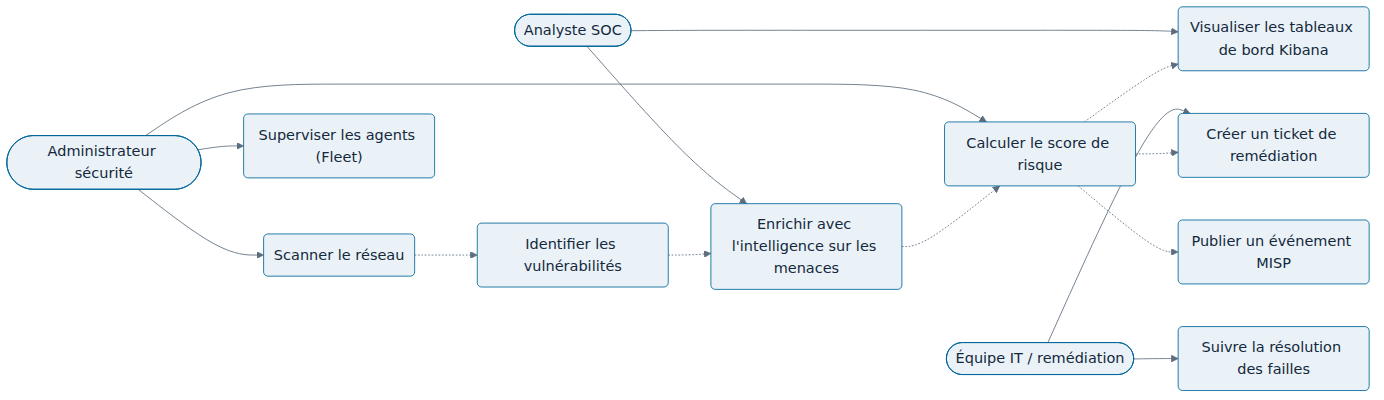
\includegraphics[width=0.62\linewidth,keepaspectratio]{diagrams/use_case.png}
\caption{Diagramme de cas d'utilisation de la plateforme VOC}
\end{figure}

Les acteurs identifi\'es sont :

\begin{itemize}[leftmargin=1.6em]
  \item \textbf{Administrateur s\'ecurit\'e} : d\'eclenche les scans, valide
        les scores et administre les agents via Fleet ;
  \item \textbf{\'Equipe IT / rem\'ediation} : traite les tickets ouverts et
        confirme la r\'esolution ;
  \item \textbf{Analyste SOC} : consulte les enrichissements et les tableaux
        de bord.
\end{itemize}

\subsection{Diagramme de classes}

Le diagramme de classes pr\'esente la structure du module des workers Celery,
avec les principales classes et leurs relations :

\begin{figure}[htbp]
\centering
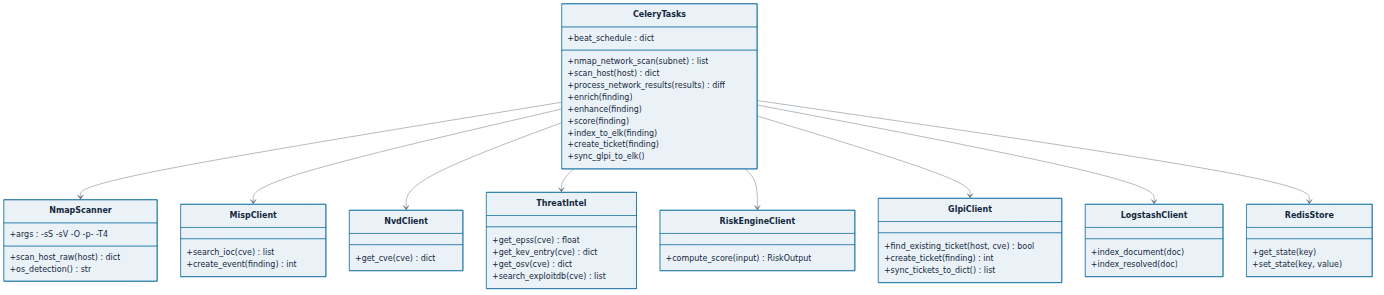
\includegraphics[width=0.78\linewidth,keepaspectratio]{diagrams/class.png}
\caption{Diagramme de classes du module workers}
\end{figure}

La classe centrale \texttt{CeleryTasks} orchestre les t\^aches du pipeline et
d\'el\`egue aux clients externes (\texttt{MispClient}, \texttt{NvdClient},
\texttt{ThreatIntel}, \texttt{RiskEngineClient}, \texttt{GlpiClient},
\texttt{LogstashClient}) ainsi qu'\`a la brique de scan
(\texttt{NmapScanner}) et au stockage d'\'etat (\texttt{RedisStore}).

\subsection{Diagramme de s\'equence}

Le diagramme de s\'equence d\'etaille l'\'echange de messages lors d'un cycle
de scan et de traitement d'une vuln\'erabilit\'e :

\begin{figure}[htbp]
\centering
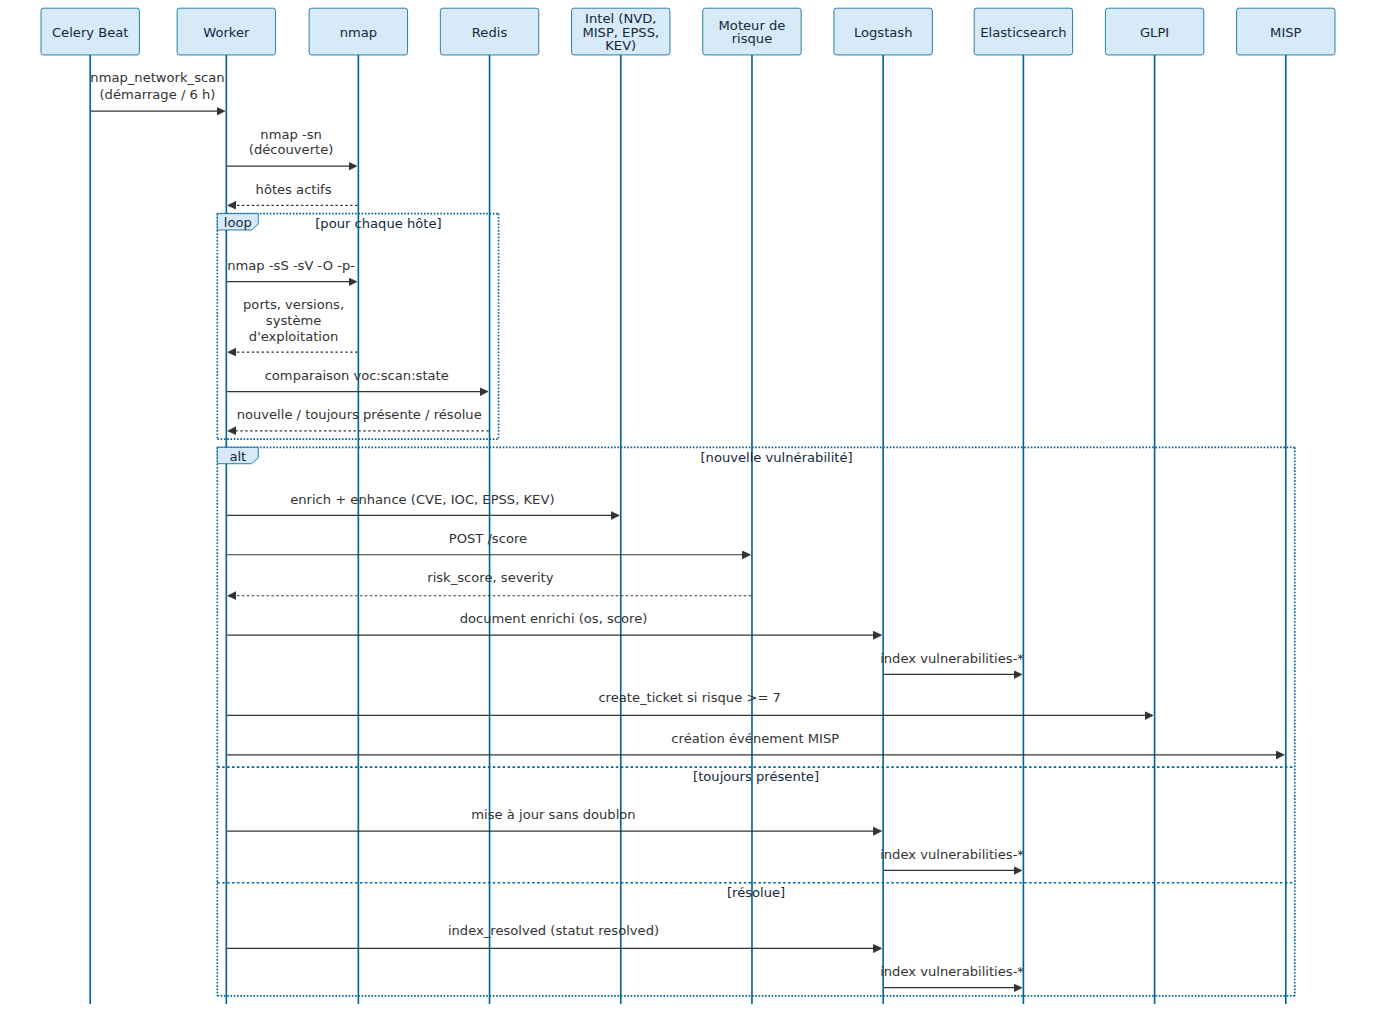
\includegraphics[width=0.9\linewidth,keepaspectratio]{diagrams/sequence_scan.png}
\caption{Diagramme de s\'equence du cycle de scan et de traitement}
\end{figure}

\subsection{Diagramme d'\'etats}

Le diagramme d'\'etats illustre le cycle de vie d'une vuln\'erabilit\'e, de sa
d\'ecouverte \`a sa r\'esolution :

\begin{figure}[htbp]
\centering
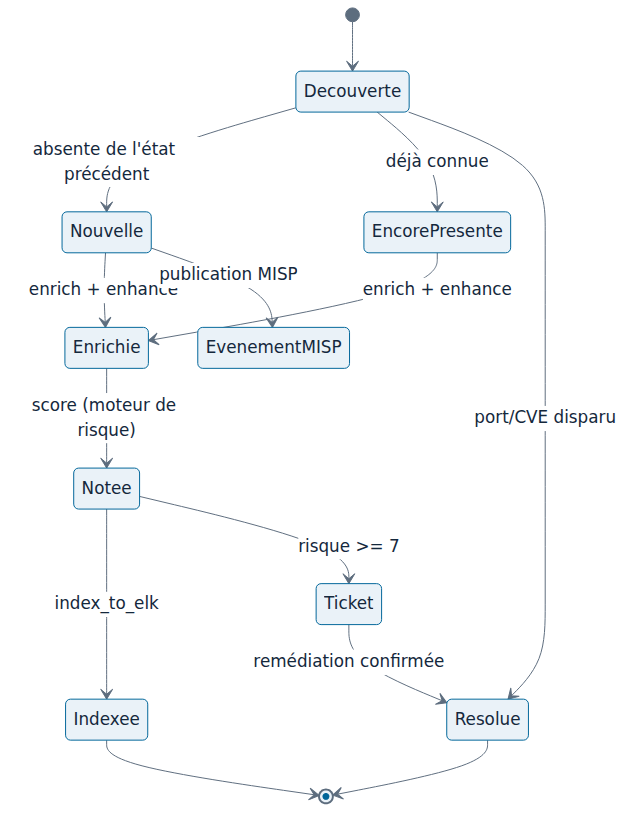
\includegraphics[width=0.62\linewidth,keepaspectratio]{diagrams/state.png}
\caption{Diagramme d'\'etats du cycle de vie d'une vuln\'erabilit\'e}
\end{figure}

\subsection{Diagramme de d\'eploiement}

Le diagramme de d\'eploiement pr\'esente la r\'epartition physique des
composants sur l'h\^ote VMware et les h\^otes externes :

\begin{figure}[htbp]
\centering
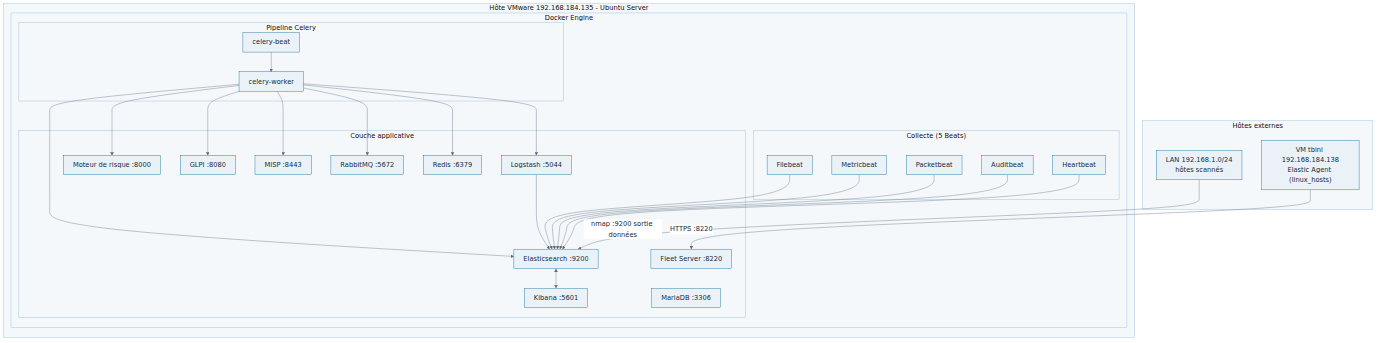
\includegraphics[width=0.78\linewidth,keepaspectratio]{diagrams/deployment.png}
\caption{Diagramme de d\'eploiement de la plateforme}
\end{figure}

\clearpage
